% Introduction

\chapter{Introduction} % Main chapter title

\label{Introduction} % For referencing the chapter elsewhere, use \ref{introduction} 

%----------------------------------------------------------------------------------------

% Define some commands to keep the formatting separated from the content 
\newcommand{\keyword}[1]{\textbf{#1}}
\newcommand{\tabhead}[1]{\textbf{#1}}
\newcommand{\code}[1]{\texttt{#1}}
\newcommand{\file}[1]{\texttt{\bfseries#1}}
\newcommand{\option}[1]{\texttt{\itshape#1}}

%----------------------------------------------------------------------------------------

It is far from our imagination to relate our everyday life with the scientific discoveries in High-Energy Physics. Still, a deep dive into these results would show us the tight bond between the smallest components of our surrounding world and their interactions with each other. The extraordinary advancements and innovations together with the development and implementations of technologies in the Large Hadron Collider (LHC) and its connected experiments have yielded incomparable and unmatched discoveries in the realm of high-energy physics. Over the years, since the inception of the world's largest collider, this collective effort has not only uncovered numerous scientific mysteries but also marked a transformative era in the field.\\

Among all the many primary active (and to be started) experiments located at LHC, the ATLAS experiment had a major role in the remarkable discoveries which was made in LHC. The infamous ATLAS, which stands for 'A Toroidal LHC ApparatuS', is the largest particle detector located at LHC, and a complex and multi-purpose detector, focused on a range of topics to improve our perception of the fundamental components of matter.\\
The ATLAS experiment is inherently designed to address several key objectives within particle physics. These include the study and identification of the particles predicted by the Standard Model, analysis of fundamental particle interactions and the governing forces involved, and a comprehensive exploration of antimatter properties. Furthermore, the project exploits the more unexplored realms and more undiscovered topics particularly the nature of dark matter and studying the possible candidate particles, recreating the conditions of the early universe to discover the unification of the forces in extremely high energies.\cite{ATLASweb}\\

ATLAS experiment stands as an extensive collaborative initiative in the field of physical sciences, formed by one of the most extensive scientific joint efforts. It involves the active participation of over 3,000 scientists and students from over $174$ universities and laboratories and $38$ countries.\\
LHC, as the world's most powerful particle accelerator and the main engine of ATLAS and several other experiments, spanning a circumference of approximately $27 \si{\kilo\meter}$, is able to accelerate the protons to nearly the speed of light within this immense ring and form head-on collisions up to the energy of $13 \si{\tera\eV}$, in HEP known as '\textit{events}', enabling the experiments, especially ATLAS, to investigate the spectacular events detected in the head-on collisions of protons in the middle of the ATLAS detector.\cite{Barnett_2011}\\

In order to detect the produced particle and identify the reactions inside the collisions, it is necessary to measure and detect various properties of these particles. The key objectives of the detections are: Tracking the trajectory of particles, Measurement of momentum, Measurement of energy, Vertex reconstruction, and Event Timing.\\

The ATLAS detector consists of numerous parts, namely the Inner Detector (ID), Calorimeter, Muon Spectrometer (MS), Magnet system, and Trigger system, to be able to measure almost all the particle properties mentioned above, within each collision. The massive detector is built in a cylindrical shape with the dimensions of $46 \si{\meter}$ in length and $25\si{\meter}$ in diameter, with the approximate weight of $7000$ Tonnes, and placed about $100 \si{meter}$ below the ground level (Fig.\ref{fig:ATLASdetector}).\footnote{For additional and  more information about the \href{https://atlas.cern/Discover/Detector/Calorimeter}{Calorimeters}, \href{https://atlas.cern/Discover/Detector/Muon-Spectrometer}{Muon Spectrometer}, \href{https://atlas.cern/Discover/Detector/Magnet-System}{Magnetic system}, and \href{https://atlas.cern/Discover/Detector/Trigger-DAQ}{Trigger and Data Acquisition} please read @ \href{https://atlas.cern/}{ATLAS Experiment} }

\begin{figure}[h]
    \centering
    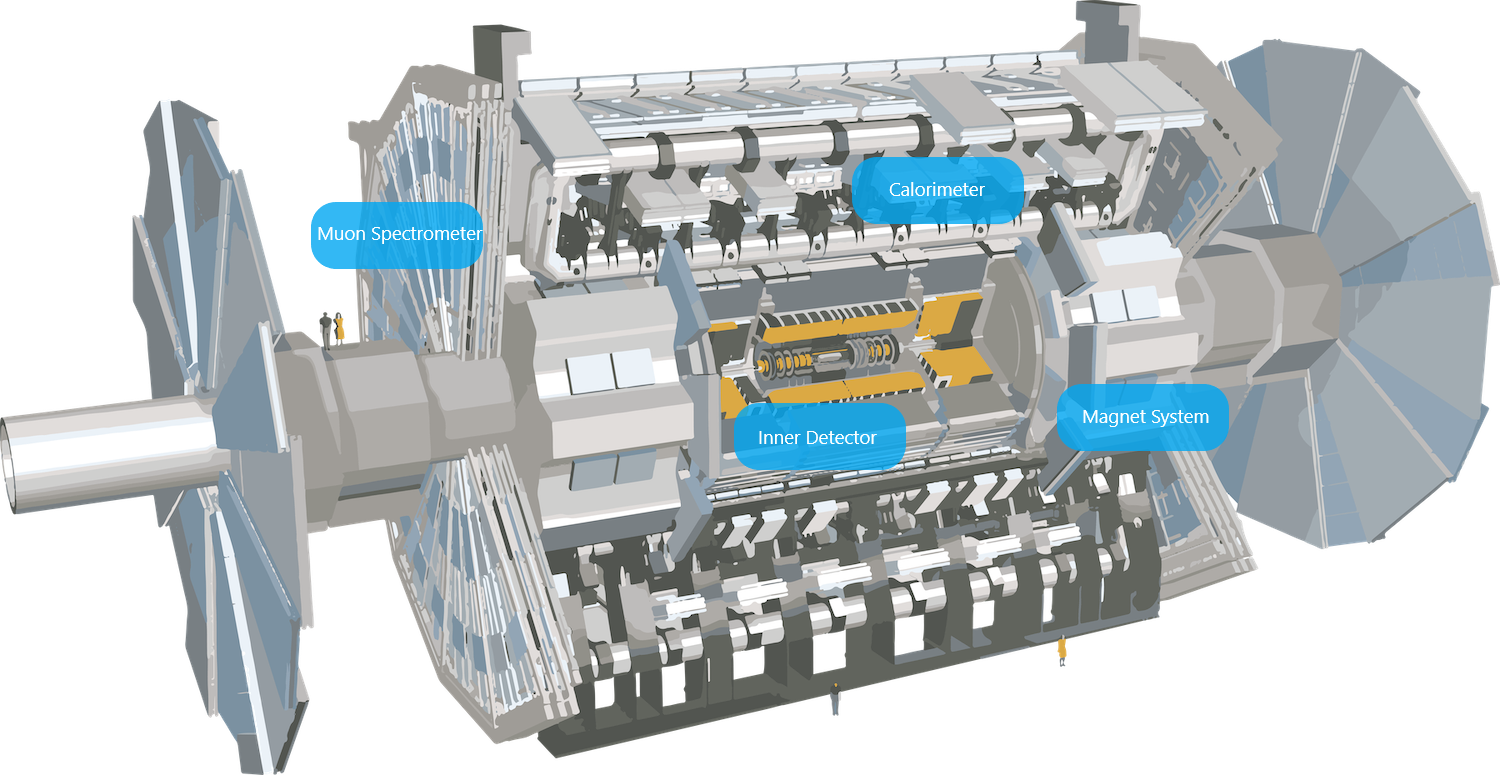
\includegraphics[width=10cm,height=7cm,keepaspectratio]{Figures/Intro/Detector reduce.png}
    \caption{The schematic view and length-wise cross-section of the ATLAS detector consisting of the Magnetic system, Inner detector, Calorimeter, and Muon Spectrometer, and showing the scale of the detector compared to a human. ATLAS Experiment  \copyright 2024 CERN}
    \label{fig:ATLASdetector}
\end{figure}

After each proton-proton collision energized by LHC inside the ATLAS detector, various processes take place to detect and analyze the produced particles and their interactions.\\
The first interaction of the produced particles with the detector takes place at the Inner Detector, positioned closest to the interaction point where proton-proton collisions occur. The currently installed and commissioning inner detector, consists of three components namely the Pixel Detector, Semiconductor Tracker (SCT), and Transition Radiation Tracker (TRT), is highly sensitive and rather smaller in size compared to the Calorimeters and Muon Spectrometer, and has a responsibility of the identification of electrons, photons, muons, and tau-leptons produced in both heavy-ion collisions and proton-proton interactions, as well as charged-particle reconstruction and heavy-flavour tagging. Additionally, it is used for reconstructing the trajectories of charged particles and is utilized in pile-up vertices and pile-up jet rejection, identification of primary and secondary vertices, complete reconstruction of exclusive decay modes, tracking of interactions and photon conversions, and particle identification through transition radiation and $dE/dx$. \\
The current ATLAS Inner Tracking Detector was designed to operate at a $14  \si{\tera\eV}$ center-of-mass energy, an average pile-up of $23$ proton-proton interactions per crossing\footnote{The term "proton-proton interaction per crossing" describes the number of interactions or collisions that take place between protons each time a proton beam crosses over another at a particle accelerator's collision site. Protons travel in opposing directions and collide at certain points of interaction when used in experiments at facilities like CERN's LHC. More @ \href{https://lhc-machine-outreach.web.cern.ch/collisions.htm}{LHC Machine outreach}}, and a constant instantaneous luminosity of $L = \num{1e34} \si{\square\per\centi\meter\per\second}$. Later in operation, it exceeded the average pile-up of $24.2$ and the peak instantaneous luminosity of $L = \num{1.37e34}. \si{\square\per\centi\meter\per\second}$\cite{Collaboration:390920}

%commented section about the other parts of the detector
\begin{comment}
    

The Calorimeter has the responsibility of measuring the energy of the particles. The calorimetry system in the ATLAS detector consists of the Liquid Argon (LAr) Calorimeter (Electromagnetic Calorimeter) and the Tile Hadronic Calorimeter (Fig.\ref{fig:detectorAppendix}). The particles interact, are absorbed, and finally converted into a shower of lower energy particles by the high-density material in the Electromagnetic calorimeters. As a result of this process, the 'new' particles ionize the liquid Argon producing an electric current that can be measured and the cumulative currents show the energy of the original particle. The Hadronic Calorimeter has a similar functionality, but due to its design which consists of several layers of steel and plastic scintillating tiles, interacts with the Hadronic particles, which do not deposit all of their energy in the LAr Calorimeter.\\
The outmost layer is where the Muon Spectrometer is placed. Muons are unique in their ability to penetrate dense materials, and they carry information about particles that might be missed by the inner layers of the detector. Muon Spectrometer consists of five different detector technologies: Thin Gap Chambers, Resistive Plate Chambers, Monitored Drift Tubes, Small-Strip Thin-Gap Chambers, and Micromegas, allowing us to spot and measure the momentum of muons (Fig.\ref{fig:detectorAppendix}).\\
Finally, the Magnetic System provides a magnetic field to precisely measure particle momenta. This feature helps for a better understanding of particle energies and collision dynamics (Fig.\ref{fig:detectorAppendix}). The Triggering System mainly selects interesting collision events and filters them from the enormous amount of data, managing the data inquisition and preventing it from overflowing. Together, these systems enhance the efficiency and precision of the ATLAS detector at the LHC.\cite{ATLASweb}\\
 A schematic view of the particle detection, shortly explained above, is shown in Fig.\ref{fig:ATLASlayers}.

\begin{figure}[h]
    \centering
    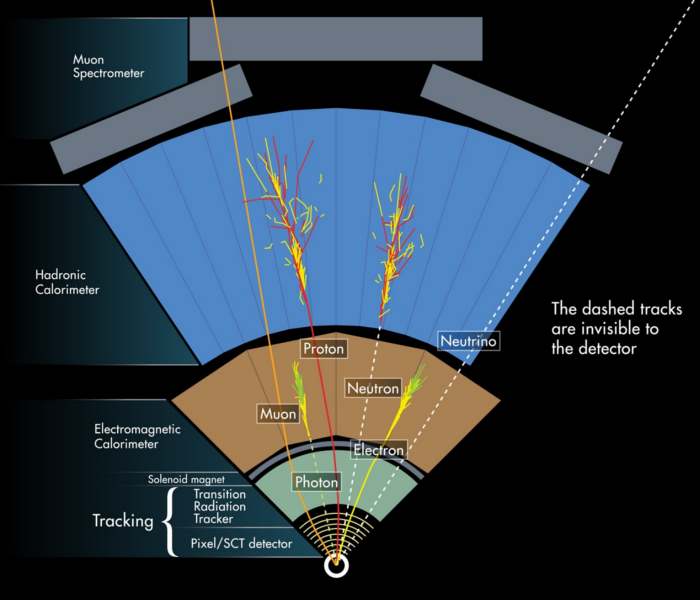
\includegraphics[width=10cm,height=10cm,keepaspectratio]{Figures/Intro/layers.png}
    \caption{An illustrated view of particle detection in the ATLAS detector, showcasing layers of different instruments. Inner detectors trace charged particle paths, calorimeters measure energy deposition, and muon detectors identify and track penetrating muons. This comprehensive system unveils the intricate details of high-energy particle interactions. \href{http://collider.physics.ox.ac.uk/}{Collider}\copyright University of Oxford, 2016 }
    \label{fig:ATLASlayers}
\end{figure}
\end{comment}

As the ongoing and anticipated discoveries within the project continually generate new questions, it drives us to further investigations and explore new areas. As a result, it becomes necessary to design and upgrade detectors. We ensure that we stay at the forefront of scientific investigation and meet the changing needs of our research by improving our detecting skills. The Inner Tracker upgrade gives us more accuracy and capacity to record the finer details of particle interactions. We can push the limits of our knowledge owing to this constant progress, which has helped us make important advancements in high-energy physics. The inner tracker is undergoing a major upgrade to make this goal possible. The goals of the ITk upgrade project include improving tracking precision, handling higher particle fluxes, and ensuring the detector's resilience in the challenging environment of the upgraded High-Luminosity LHC (HL-LHC), which will provide even more intense beams of protons. It is expected to achieve an average of $140$–$200$ inelastic proton-proton collisions per crossing, with the instantaneous luminosities of $L = 5-\num{7.5e34} \si{\square\per\centi\meter\per\second} $ at a $14  \si{\tera\eV}$ center-of-mass energy. This design promises a total data set of $4000 \si{\per\femtobarn}$ \footnote{"\textit{Integrated luminosity is usually expressed in units of “inverse femtobarns” ($\si{\per\femtobarn}$). A femtobarn is a unit of cross-section, a measure of the probability for a process to occur in a particle interaction. This is best illustrated with an example: the total cross-section for Higgs boson production in proton–proton collisions at $13 \si{\tera\eV}$ at the LHC is of the order of $6000\si{\per\femtobarn}$. This means that every time the LHC delivers $1\si{\per\femtobarn}$$ of integrated luminosity, about $6000 \si{\per\femtobarn}$ x 1 $\si{\femtobarn} = $6000$ Higgs bosons are produced.}"\cite{CERNweb}} over the $10$ years of prospective operation time of the new ATLAS ITk detector. \\

The new detector consists of multiple layers of silicon particle detectors; Silicon microstrip sensors will make up the outermost layers, with four concentric barrel layers and one end-cap section featuring six disks on each barrel side, while silicon pixel sensors will form the innermost layers. The Long Strip modules (LS modules) with $48.35 \si{\milli\meter}$ strips length are placed in the outer two barrel layers, while the Short Strip modules (SS modules) with parallel strips length of $24.16 \si{\milli\meter}$ length are housed in the inner two barrel layers. Six disks per side, with trapezoidal-shaped sensors of varying lengths and strip pitches, make up the forward portions of the end-cap strip tracker.  This new design is expected to endure the extremely harsh radiation environment, which the current inner detector is vulnerable to at Pixel detector, Semiconductor Tracker (SCT), and Transition Radiation Tracker (TRT), by substituting the electronic parts of the older design with hybrid silicon pixels, providing $3$ times more silicon area of the current ID, and lowering the risk of the damaging the sensor due to the high radiation.\cite{herde2023atlas}. Figure \ref{fig:ITklayout} shows the schematic view of the layout of the Inner Tracker and the main detector's components.\\

\begin{figure*}[h]
    \centering
    \begin{subfigure}[t]{0.45\textwidth}
        \centering
        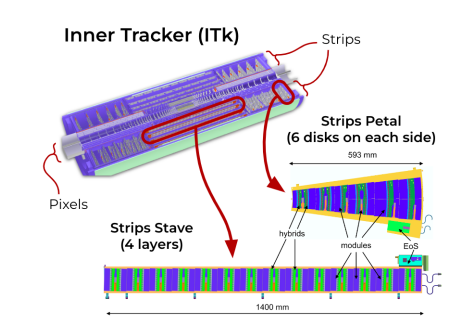
\includegraphics[height=4.5cm]{Figures/Intro/component.PNG}
        \caption{} \label{fig:ITklayout1}
    \end{subfigure}
    ~ 
    \begin{subfigure}[t]{0.45\textwidth}
        \centering
        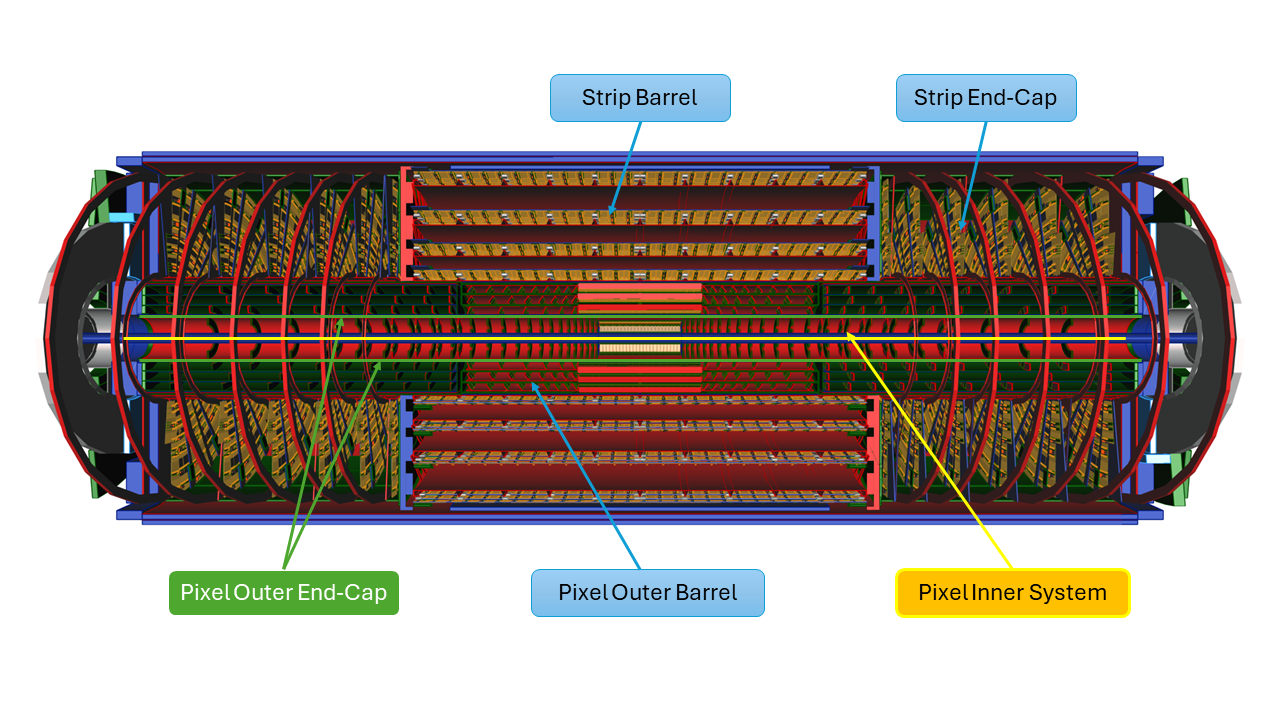
\includegraphics[height=4cm]{Figures/Intro/fig_07Edited.png}
        \caption{}
        \label{fig:ITklayout2}
    \end{subfigure}
    \caption{a) A schematic view of ITk showing the pixel detector surrounded by a Strip Detector Picture from \cite{itkcomponent}, and b) Cross-section view of the Inner Tracker showcasing the Strip barrel, Strip end-cap, Pixel outer end-cap, Pixel outer barrel, and Pixel inner system. Picture from \cite{ATL-PHYS-PUB-2021-024}} 
    \label{fig:ITklayout}
\end{figure*}





As the precision and consistency of the acquired data are directly dependent on these modules, it is crucial to perform various rigorous tests to spot any potential glitches or deviations in performance that might compromise the integrity of experimental outcomes. With ATLAS ITk modules serving as the primary data collectors in the critical particle collision environment at the LHC, reliability testing of these components is essential, to ensure that each module operates at peak efficiency, minimizing data inaccuracies and strengthening the reliability of scientific findings.\\
Since the scope of the upgrade project is very big and beyond any single institute to cover all aspects of the project, it requires close collaboration between multiple research institutions, laboratories, and experts in various fields, and the testing part of the ITk module production indeed requires the collaboration of several scientific institutes. However, the information and the data stream related to each part of the test have to be consistent and cover all the required data for further analysis and probing. This thesis focuses on the reliability testing of ATLAS ITk modules, and its primary goal is to conduct thorough and rigorous tests to identify potential vulnerabilities, weaknesses, or variations in performance by tracking the performance in different environmental and experimental situations, the stability of the components and data handling, and quality control of the modules specifically for the long-term usage. The project mainly consists of $4$ different parts: 
%edit this better
\begin{itemize}
    \item an attempt to add additional information to the test data
    \item establishing a connection to the database to store the data for further analysis proficiently
    \item setting up a test environment and performing the long-term reliability tests
    \item analyzing the data gathered by the tests
\end{itemize}

Given that there is no turning back once the modules are installed, it emphasizes the importance of carrying out extensive long-term reliability testing. Identifying their optimal functionality and dependency is crucial, as any doubts or problems that arise after installation would be permanent. This proactive approach reduces the possibility of unanticipated issues and gives stakeholders confidence that the modules will function seamlessly and dependably in their assigned roles.\\

Subsequently, readers can expect to delve into a comprehensive exploration of the mentioned topic, beginning with an introduction to the test setup, including the configuration and instrumentation utilized to conduct the tests. Additionally, we will outline the different executable controlling systems of the tests, as well as methods of storing and merging the data gathered from the data for further analysis. Lastly, we present the results from the long-term reliability test of the modules, perform a comprehensive analysis of the test data, and preview the validity of the quality of the manufactured modules. 
%write a bit about this text being a reference for text
%add a bit more on HL-LHC and less about modules. 
%Add itk layout: layout of pixel and strips